\section{Results and Discussion}
	In the section the classification that took place will be analyzed. The classification were conducted in different configurations of  dataset size and number of features. For optimization purposes other characteristics will be discussed such as robustness of the results as well as training and classification time.
	
	\subsection{Grouping of Classifiers}
		The classifiers were grouped into 5 general groups. Additionally, a Vote Classifier, tallying the voted classifications was observed. The groupings were done according to the base algorithm of each classifier. This organization schema is demonstrated in Table \ref{table:class_grps}.
		
		\begin{table}[h]	
			\begin{center}
				\begin{tabular}{c |c| l} 
					\hline
					\hline
					\multicolumn{1}{c|}{\multirow{2}{*}{Group Name}} & \multicolumn{1}{|c}{\multirow{2}{*}{Abbreviation}} & \multicolumn{1}{|c}{\multirow{2}{*}{Classifiers}}\\ 
					 &&   \\ 
					\hline
					Regressions 	  && Logistic Regression*  \\
					\hline
					\multirow{2}{*}{Naive Bayes} & \multirow{2}{*}{NB} & Simple NB, Bernoulli NB,\\
					       	  & & Multinomial NB \\
					\hline
					\vspace*{-1mm} 
					\multirow{3}{*}{\begin{tabular}{@{}c@{}}Support Vector \\ Machines \end{tabular}}  
					 &\multirow{3}{*}{SVM}& Linea Kernel, Polynomial Kernel,\\
									  && Radial Basis Function Kernel,\\
							  &&  Sigmoid Kernel \\
					\hline
					\vspace*{-1mm} 
					Artificial Neural &\multirow{2}{*}{ANN}& Multi-Layer Percpetron,  \\
					Networks		  && Stochastic Gradient Descent** \\
					\hline
					Ensemble Methods  &Ensembles& Random Forest, Adaptive Boosting \\
					\hline\hline
					\multicolumn{3}{p{1\textwidth}}{ \footnotesize * Note that Logistic Regression refers to a classification schema using logistic distribution for possible values of the fore-casted class, rather then an actual regression. Furthermore, Logistic Regression is a simplistic classifier and is demonstrated as a benchmark measure, rather then an actual classifier.} \\
					\multicolumn{3}{p{1\textwidth}}{ \footnotesize ** Refers to Neural Networks which make use of SGD to minimize their cost function by gradually reducing the error terms} \\
				\end{tabular}	
			\end{center}
			\caption[Classifier Groupings]{Classifier Groupings}
			\label{table:class_grps}
		\end{table}
	
		In the upcoming results analysis the name scheme used in Table \ref{table:class_grps} will refer to average values inside each such named group. 
	
	\subsection{Approaches}
		\label{section:feature_types}
		\subsubsection{Descriptive Features}
			\label{section:Descriptive_Features}
			Similar approaches were used to classify Information Credibility on Tweeter (\cite{castillo2011information}). In some sense, the mission of this study is also to quantify the quality of social media content, however, in a very subjective manner.
			\par	
		
			Every Tweet object originating from the Twitter database is a complex multi-layered structure, which  simultaneously describes the posted Tweet itself along with the user profile of its author and any additional media objects related to the Tweet. This approach to feature extraction focuses on deriving the implicit meaning or sense of the tweet, rather than analyzing the verbatim textual content. As previously noted in Section \ref{section:Descriptive_Features}, two tiers of features are extracted. The former type describes the Tweet object, whereas the latter draws information about the author himself. These features are described in Table \ref{table:desc_features} and are explained in the following paragraphs. Appendix \ref{appn:desc_features_stats} describes the general statistics of these features. 
			
			\begin{table}[h]	
			\begin{center}
				\resizebox{1 \textwidth}{!}{
				\begin{tabular}{c |l| l} 
					\hline
					\hline
					\multicolumn{1}{c|}{\multirow{2}{*}{Scope}} & \multicolumn{1}{|c}{\multirow{2}{*}{Feature}} & \multicolumn{1}{|c}{\multirow{2}{*}{Description}}\\ 
					&&   \\ 
					\hline
					\multirow{17}{*}{Message}& NUM\_STOP\_WORDS & Number of Stop-Words in the Tweet  \\
							& DUPLICATE					& An almost identical tweet was captured in same query  \\
							& LEN\_CHARACTERS			& Number of characters in Tweet text  \\
							& NUM\_WORDS				& Number of words in Tweet Text \\
							& HAS\_QUESTION\_MARK		& Tweet contains question mark  \\
							& HAS\_EXCLAMATION\_MARK	& Tweet contains exclamation mark  \\
							& HAS\_MULTI\_QUEST\_EXCLAM & Tweet contains either multiple question marks or exclamation marks \\
							& EMOJI\_SENT				& Sentiment of emoji symbols. TRUE for positive \\
							& EMOJI\_SENT\_SCORE		& Sentiment score magnitude of emoji symbols. Always non-negative  \\
							& HAS\_PRONOUN				& Tweet contains pronouns \\
							& COUNT\_UPPER				& Percent of upper case letters out of Tweet text \\
							& HAS\_HASHTAG				& Tweet contains Hashtags\\
							& RETWEET\_COUNT			& The number of times the Tweet was reposted\\
							& URLS\_WIKI				& The Tweet contains a URL, belonging to Wikipedia's top 100\\
							& URLS\_MOZ					& The Tweet contains a URL, belonging to Moz's top 500\\
							& SENTIMENT					& Tweet's sentiment score\\
							& SENTIMENT\_CONF			& Tweet's sentiment score confidence level\\
					\hline
					\multirow{8}{*}{User}	& REG\_AGE 	& Number of days since user registered on Twitter\\
							& STATUS\_CNT 				& Number of Status changes			\\
							& FOLLOWERS\_CNT 			& Number of Followers the user has	\\
							& FRIENDS\_CNT				& Number of Friends the user has	\\
							& VERIFIED					& Whether User account is verified by Twitter\\
							& HAS\_DESC 				& Whether User account contains a description\\
							& HAS\_URL					& Whether User account has a homepage URL	\\
							& MSG\_P\_DAY 				& Average number of messages posted per day	\\
					\hline\hline
				\end{tabular}
				}	
				\end{center}
				\caption{Descriptive Features}
				\label{table:desc_features}
			\end{table}
		
		
			\paragraph{Number of Stop-Words}
				The total number of Stop-Words in the tweets' text. Stop-Words are words, which carry grammatical meaning but usually little to no contextual weight. These words are also usually the most common words in the corpus. The full list of Stop-Words is available in Appendix \ref{appn:stop_words}.
				
			\paragraph{Duplicate}	
				Tweets are queried from the servers using a search term. This feature will receive the value \textit{TRUE}, if another Tweet was found, which has a similarity score exceeding a predetermined threshold. The similarity of each pair of Tweets was calculated using the S\o rensen-Dice coefficient as in Figure \ref{fig:sorenson_dice}.
			
			\paragraph{Emoji Sentiment}
				All Emoji symbols are extracted from the Tweet and are scored according to the chart in the following URL: \url{http://kt.ijs.si/data/Emoji_sentiment_ranking/}. The ranking is based on a study by \cite{Kralj2015emojis}. In this paper, Emojis were labeled to have a positive, negative or neutral connotation. The feature EMOJI\_SENT denotes the sign of sentiment (positive or negative), whereas the feature EMOJI\_SENT\_SCORE denotes the strength of the sentiment. When several Emojis are found, their appropriate values are averaged out. 
				
			\paragraph{Retweet Count}
				Twitter content can be reposted as part of a new Tweet. This operation is named \textit{retweeting} in the Tweeter nomenclature. When a Twitter user wishes to reference another Tweet in its entirety, the enclosed (Retweet) Tweet will be framed inside the new Tweet and called a Retweet. Additionally, the original post keeps track tracks of the number of times it was reposted by other users. This acts as a measure of the Tweet's diffusion.
				
			\paragraph{Popular Domains}
				Tweets often contain links to objects both inside and outside the Tweeter realm. External items are usually sourced using a Uniform Resource Locators (URL). These URLs, in turn, belong to domains. The features URLS\_WIKI and URLS\_MOZ denote whether an enclosed URL belongs to one of the top 100 or top 500 most visited domains accordingly. The list of domains are publicly available and are regularly updated. Top 100 most popular domains by Alexa are available on Wikipedia: \url{https://en.wikipedia.org/wiki/List_of_most_popular_websites} and the top 500 most popular domains are provided by MOZ on \url{https://moz.com/top500}.
			
			\paragraph{Tweet Sentiment}
				The NLTK corpora contains a set of 10,000 Tweets labeled per hand to have either a positive or negative sentimental connotation. A Machine-Learning algorithm was trained using this set, to classify Tweets their sentiment. The classification in done using a Vote classifier. The feature SENTIMENT denotes the Tweet's sentiment (TRUE for positive or FALSE for negative) and SENTIMENT\_CONF denotes the number of underling classifiers of the Vote classifier, which voted for the aforementioned label.
				
			\paragraph{Status Count}
				On the Tweeter platform every post by submitted is regarded as a new \textit{Status} or a \textit{Status Change}. The feature indicated the number of such Statuses since the inception of the Tweeter account. This number includes both Tweets and Retweets.
			
			\paragraph{Verified}	
				User accounts are usually not limited when choosing a moniker to go by publicly on Tweeter. This leads to a plethora of accounts impersonating figures or organizations of public interest. Tweeter tries to verify the authenticity of accounts, which it is determines to be of public interest (see: \url{https://support.twitter.com/articles/119135}). Figure \ref{fig:verified_accounts} demonstrates a verified and a unverified Tweeter account of U.S. president Donald J. Trump. \textit{Source: Twitter}

				
				\begin{figure}[h]
					\centering
					\captionsetup{width=0.8\textwidth}
					\includegraphics[width=0.8\textwidth]{verified_account.png}
					\caption[Tweeter Verified Accounts]{
						\footnotesize{
							Tweeter verified (left) and unverified (right) accounts of U.S. president Donald J. Trump. Notice the blue badge denoting a verified account next to the profile name.
						}
					} 
					\label{fig:verified_accounts}
				\end{figure}
			
			\paragraph{Followers Count}
				The number of Tweeter users actively following this user. A high number of followers suggests, that the person may be views as an Opinion Leader or a person whose carries substantial influence on social media.
				
			\paragraph{Friends Count}
				This features is the mirror image of the Followers Count. It specifies the number of User accounts the current User is following.
					
		\subsubsection{Bag-of-Words}
			This approach simply converts the entire text corpus to a frequency charts of all the words contained within. Words are then selected to act as features in incoming data, which is to be classified. The features are hence a variable list (usually of several thousands in length), where each variable is a boolean representation, indicating the presence or absence of a certain word. Usually the words undergo preprocessing as is common in Natural Language Processing prior to being used as features. The corpora are segmented to lists of words, often omitting articles, proposition and punctuation. Such grammatical structures are critical in human speech and written form in order to convey one's meaning clearly and explicitly, however for the purposes of more ambiguous classification as in our case, such nuances are avoided for the sake of simplicity. Words are then \textit{stemmed} or \textit{lemmatized}, meaning their are reverted to their grammatical stem - dropping all prefixes and suffixes. This eases the enumeration of words, since it is preferable that the same words in different inclinations would be counted as the same. For example, the word pair \textit{eating} and \textit{ate} would be reverted to their stem \textit{eat}, as well as \textit{apple} and \textit{apples} would be considered as one and the same. Finally, words would be assigned their part of speech (noun, verb, adjective ..) and could be either ignored or incorporated into the feature set, according to the conceived importance of a given part of speech.
		
			Therefore, this technique draws meaning from the verbal content of a corpus. From another perspective, one might say that each word carries certain information towards distinguishing different text samples along some trait. We strive to draw correlations between frequencies of certain words and classes to which, we wish to label the samples. Table \ref{table:BOW_top_words} shows most frequent words to be encountered in the corpus. 
			
			\begin{table}[H]
				\centering
				\begin{tabular}{ccc}
					\hline\hline
						&	Word 	& Frequency \\
					\hline
					1	&	amazon 	& 1857	\\
					2	&	food	& 248	\\	
					3	&	whole 	& 212	\\
					4	&	new		& 199	\\
					5	&	book	& 183	\\
					6	&	amp		& 161	\\
					7	&	echo 	& 155	\\
					8	&	free 	& 130	\\
					9	&	buy 	& 124	\\
					10	&	prime 	& 113	\\
					\hline\hline				
				\end{tabular}
				\qquad 
				\begin{tabular}{ccc}
					\hline\hline
					&	Word 	& Frequency \\
					\hline
					7889	&	medieval 		& 1	\\
					7890	&	npr				& 1	\\	
					7891	&	katerichards09 	& 1	\\
					7892	&	champ			& 1	\\
					7893	&	prosecutor		& 1	\\
					7894	&	khalids			& 1	\\
					7895	&	explains 		& 1	\\
					7896	&	commenting 		& 1	\\
					7897	&	george 			& 1	\\
					7898	&	lowcost 		& 1	\\
					\hline\hline				
				\end{tabular}
				\caption{Top 10 Most and Least Frequent Words Captured}
				\label{table:BOW_top_words}%
			\end{table}%
		
		\subsubsection{N-Grams}
			A development on the Bag-of-Words concept. Using this approach, sequences of $ n $ words are extracted instead of single words and used as features. Such an approach has the added benefit of preserving some of contextual meaning of the text as well as discovering reoccurring phrases. This would prove even more beneficial is scenarios, in which the classification would be between positive and negative intonation, such as opinions and reviews. A down side to this method, is that much more feature are created therefore increasing the computational complexity. 
			
			\begin{table}[h]	
				\begin{center}
					\begin{tabular}{c l} 
						\hline\hline
						N &  \multicolumn{1}{c}{Possible N-Grams }  \\ 
						\hline
						2 & the movie ; movie was ; was not ; not great  \\
						3 & the movie was ; movie was not ; was not great \\
						4 & the movie was not ; movie was not great \\
						5 & the movie was not great \\ 
						\hline\hline
					\end{tabular}
				\end{center}
				\caption[N-Gram Example]{Possible N-grams of size 2 to 5 }
				\label{table:ngrams}
			\end{table}
			
			For example, using standard Bag-of-Words approach on the sentence "the movie was not great" results in 5 features \{the ; movie ; was ; not ; great\}. When applying \textit{N-Grams} of sizes 2 to 5 on the same sentence, results in 10 features as seen in Table \ref{table:ngrams}.
			
			\begin{table}[H]
				\centering
				\footnotesize
				\resizebox{1 \textwidth}{!}{
				\begin{tabular}{c| lc | lc }
					\hline\hline
						&  \multicolumn{1}{c}{2-Grams}	& Frequency & \multicolumn{1}{c}{3-Grams} & Frequency\\
					\hline
					1	&	on amazon 	& 938 		& have just listed 		& 260 		\\
					2	&	via amazon 	& 842 		& available on amazon	& 96 		\\	
					3	&	whole foods & 366  		& 399 via amazon		& 81 		\\ 
					4	&	of the		& 333 		& for 399 via			& 81 		\\
					5	&	in the		& 300  		& panini for 399		& 70 		\\
					6	&	just listed	& 282 		& buying whole foods 	& 65 		\\
					7	&	have just 	& 265 		& on sale for			& 60 		\\
					8	&	check out 	& 223  		& whole foods for 		& 59 		\\
					9	&	amazon prime& 218		& tune in buy			& 55 		\\
					10	&	amazon echo & 163  		& buypayoff amazon amazonproducts	& 55 		\\
					\hline\hline
					 	& \multicolumn{1}{c}{4-Grams} & Frequency & \multicolumn{1}{c}{5-Grams}	& Frequency \\
					\hline
					1	&for 399 via amazon  	& 81 & 2004 panini for 399 via 			   & 50	\\
					2	& panini for 399 via 	& 70 & is now on sale for 				   & 49	\\	
					3	& tune in buy it	 	& 55 &	germany euro 2004 panini for 	   & 47	\\ 
					4	& buypayoff amazon products bestbuy	& 55 &	might like pumpkinfarmer iartg novel & 46\\
					5	& 2004 panini for 399	& 50 & amazon is buying whole foods 	   & 43	\\
					6	& euro 2004 panini for 	& 50 & amazon to buy whole foods 		   & 31	\\
					7	& is now on sale	 	& 50 & pbscale ai big data cloud 		   & 23	\\
					8	& now on sale for		& 49 & check out this amazon deal		   & 22	\\
					9	& ai big data cloud		& 46 & ai big data cloud boot 			   & 21	\\
					10	& now available on amazon& 39& looking for professional book cover & 17	\\	
					\hline	
				\end{tabular}
				}
				\caption{Top 10 Most and Least Frequent N-Grams Captured}
				\label{table:top_ngrams}%
			\end{table}% 
		
		Table \ref{table:top_ngrams} exemplifies the most and least often occurring N-Grams of sizes 2 - 5 words each. The 4-word phrase "is now on sale" appeared 50 times in the large Tweet corpus.
	
	\subsection{Descriptive Statistics}
		\label{section:Descriptive_Features}
		This method offers an alternative approach to features, differing from the other two, by being based on a more generalized view of the Tweet. Instead of concentrating on the actual textual content, other non direct properties are observed. Descriptive features are aimed at describing the Tweets implicit properties, such as attitude, sentiment, seriousness and trustworthiness. These features detect the presence of different symbols, their frequency and consecutiveness. Additionally, unlike the Word-Based approach, non-textual objects such as multimedia, links and mentions of other users and Tweets are also taken into account. Furthermore, features of a Tweets' owner are also included in the input. Since Tweeter's API provides a complete user profile incorporated inside the Tweet data object itself, constructing features describing the user is done simultaneously to features describing the content of the Tweet itself. This approach might be viewed as an \textit{indirect} one, since less obvious properties of the Tweet are used to characterize it.
		\par
		Descriptive features could be segregated into two distinctive groups. The first tier is text-based features. As the name suggests, these features will mostly denote the presence or lack of specific characters such as emoticons and signs in the Tweets text. Whether a Tweet contains combinations or sequences of certain symbols as well as ratios defining the text also befit this category.
		\par
		The second tier of features describe any special \textit{Entities} (Tweeter's nomenclature) contained within a Tweet. \textit{Entities} refer to non-textual contents of a Tweet, such as media (in form of pictures, audio or video), URL's linking to external websites, mentions or Retweets (referring to other Tweets or to Tweeter user profiles) and finally Hashtags. A word or phrase preceded by the Hashtag symbol \textbf{\#} indicates an association of web content (such as a Tweet or other micro-blogging post) to a specific theme. These could be an event, news, gossip or any other tidbit (\cite{dict_Tweet}). Hashtags are used primarily to simplify looking up Tweets or other social media content by technically associating them with the \textit{hashtagged} topic.
		
		The labeling of training examples was conducted by me personally in the process of several weeks. The labeling process was very subjective. Apart from holding up to a few rules of thumb, it is hard to formally model the labeling pattern. This in fact, makes this an ideal task for Machine Learning, since the logic behind it is intuitive rather than strict.
		
		\subsubsection{Data Size and Labels}
			The initial data set consisted of about 12 thousand labeled Tweets captured during a period of several days. The software would launch a listener, which would intercept all Tweets containing the word \textit{Amazon}. The listener was also programmed to ignore all Tweets which contain one of the following words and Expressions: \textit{gift}, \textit{giftcard}, \textit{giveaway}. These phrases were usually found in spam Tweets or Tweets posted by Bots and contained mostly advertising content. The captured Tweets were than labeled manually using custom made software. Out of the 12 thousand Tweets, about 1400 were labeled as "News" and the rest as "Not-News". These ratio between interesting and not-interesting content make practical sense as well, since we strive to boil the data down to only the most subjectively essential information. 
			
			\par
			
			Another issue with the data was trending topics. It was common for an announcement to be made about a new product or service, which would result in a major percentage of all Amazon related traffic to concentrate around the topic. For example, this was the case with the Amazon Echo device. For unclear purposes, some bots would take such an announcement Tweet, which originated from a certified publisher, and retweet it numerous times with minor adjustments to the text. This is turn, escalates the problem of the data being prone to concentrate heavily on some topics and much less on others. A classifier trained on such data is prone to overfitting.
			
			\paragraph{Overfitting}
				Overfitting is a very common issue in the classification field. this means that a classifier is trained in a matter fitting the data very specifically. Therefore, any slight deviation in the new data from the rigid constraints of the trained classifier results in misclassifications. Overfitting could also be viewed as the inability of the algorithm to generalize the rules learned from the data onto new information, which in essence is the purpose of Machine Learning Classification. To prevent this phenomena, the data should he heterogeneous in its content and properties and present as many different learning scenarios for the algorithm to learn from. Overall, overfitting is accepted to some degree in classification, since it is impossible to completely eliminate it. The alternative to overfitting is \textit{underfitting}, which means an algorithm which over simplifies and generalizes to an extent which makes classifications useless.
		
		\subsubsection{Data Sparsity}
			\label{data_sparsity}
			A property which is often encountered when researching Big Data. From a purely technical perspective, Data Sparsity (or Density) describes the amount of zeros in the data, when addressing binary attributes. Stated more simply, when data is immensely heterogeneous an often repeating feature is less likely to occur. In other words, the probability of a feature to be unique is higher. If we compare both approaches to textual features used in this work, \textit{Bag-of-Words} and \textit{N-Grams}, applying the former approach results in features indicating the presence of a single word, whereas with the latter every feature indicates the presence of a string of words. Intuitively, the appearance of a specific single word is much more likely than the appearance of several words in a specific order. For example, the single word "buy" is likely to appear in more samples than the phrase "people often buy", which is a \textit{3-Gram}. Thereupon, we one may deduce, that data is sparser for \textit{N-Grams} in comparison to \textit{Bag-of-Words}.
		
		\subsubsection{Number of Features}
			Initially, the classification simulation were conducted with the goal of reaching the most precise classifier irregardless of cost and duration. Thereby, the largest possible data set was used with 5000 features, when implementing the \textit{Bag-of-Words} or \textit{N-Grams} approach. The number of features, thus indicates the amount of sought-after words of expressions. Naturally, having more features results in more precise classifiers but at the same time incurs higher computational costs. Furthermore, the greater the training data set is, the more words must be scanned and tabulated by the algorithm, which also has an increasing effect on the computational time. An additional not obvious disadvantage to training classifiers with a large number of features is the risk of overfitting the classifier, as discussed previously. 
			
			\par
			Table \ref{table:class_duration} demonstrates the average duration in seconds to train a classifier. The training dataset size is denoted on the horizontal axis and the number of identifying features on the vertical axis. Moreover, the table is split to two parts, each representing another approach to feature construction, \textit{Bag-of-Words} and \textit{N-Grams} are positioned above and below accordingly. Notice the large standard errors, indicated by the numbers in brackets. This strong variation is due to the differences in the training time of the different algorithms. Furthermore, some algorithms (such as SVMs) entail quadratic complexity which makes them scale in a non-linear fashion, causing much longer training times. For example, training a classifier with 3000 features and a training dataset size of 2000 takes an average of 17,63 seconds with a standard error of 16,65 seconds.
			
			\par
			
			\begin{figure}[H]
				\begin{center}
					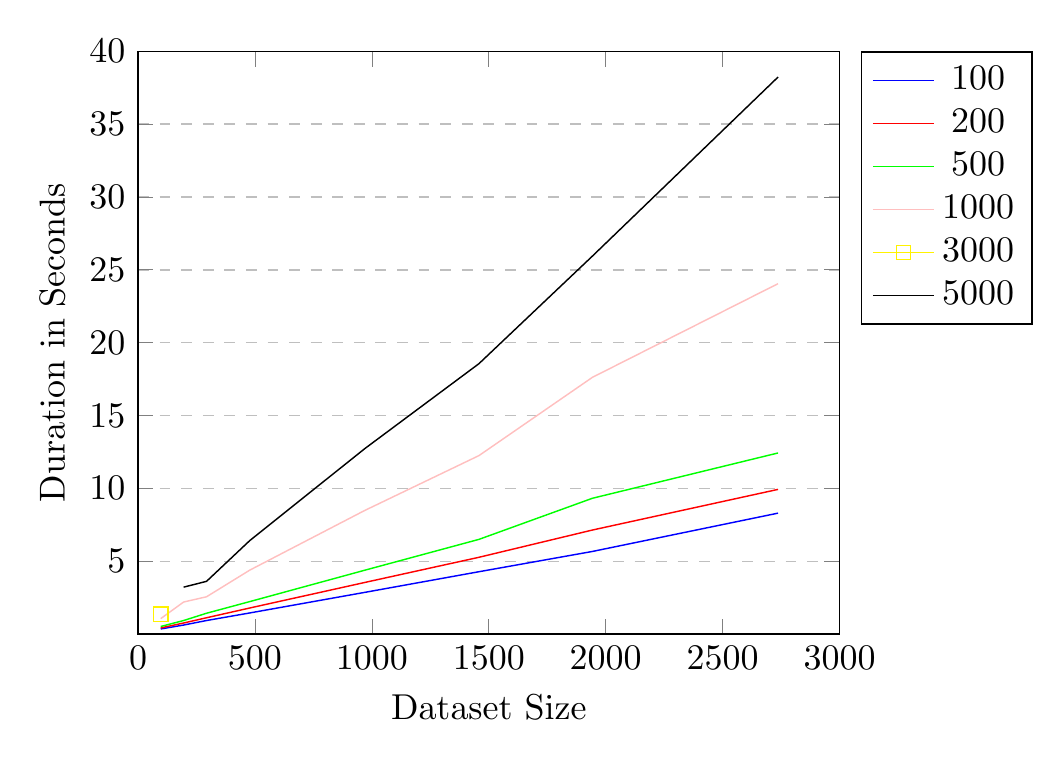
\begin{tikzpicture}[scale=1.3]
					\begin{axis}[
					/pgf/number format/.cd,
					use comma, 1000 sep={},
					xlabel={Dataset Size },
					ylabel={Duration in Seconds},
					xmin=0, xmax=3000,
					ymin=0, ymax=40,
					xtick={0,500,1000,1500,2000,2500,3000},
					ytick={5,10,15,20,25,30,35,40},
					legend pos=outer north east,
					ymajorgrids=true,
					grid style=dashed,
					]
					\addplot[color=blue,mark=no,]
					coordinates {
						(97,0.35)(195,0.62)(293,0.93)(478,1.45)(969,2.86)(1458,4.28)(1943,5.67)(2737,8.30)
					};
					\addplot[color=red,mark=no,]
					coordinates {
						(97,0.42)(195,0.76)(293,1.12)(478,1.79)(969,3.54)(1458,5.27)(1943,7.14)(2737,9.93)
					};
					\addplot[color=green,mark=no,]
					coordinates {
						(97,0.52)(195,0.93)(293,1.43)(478,2.23)(969,4.38)(1458,6.50)(1943,9.32)(2737,12.43)
					};
					\addplot[color=pink,mark=no,]
					coordinates {
						(97,1.06)(195,2.20)(293,2.56)(478,4.39)(969,8.48)(1458,12.25)(1943,17.62)(2737,24.05)	
					};
					\addplot[color=yellow,mark=square,]
					coordinates {
						(97,1.36)
					};
					\addplot[color=black,mark=no,]
					coordinates {
						(195,3.22)(293,3.62)(478,6.42)(969,12.72)(1458,18.56)(1943,25.94)(2737,38.23)
					};	
					\legend{100,200,500,1000,3000,5000}					
					\end{axis}
					\end{tikzpicture}
					\captionsetup{width=0.8\textwidth}
					\caption[Training Duration]{Training Duration as Function of Set Size and Number of Features with the Bag-of-Words Approach}
					\label{fig:duration_growth}
				\end{center}
			\end{figure} 
		
			The question of how training duration scales cannot be adequately answered within the scope of this work due to the dataset size limitation. However, the duration seems to grow in a geometric fashion as the dataset size or number of features increase. This growth is illustrated in Figure \ref{fig:duration_growth}. Nonetheless, the overall duration time seems manageable and would scale even better still when conducted on a more powerful computer. This holds especially true when implementing the mathematically simpler models (not SVMs). A more detailed view of training duration for each classifier is available in \hyperref[tab:dur_by_type]{Appendix A}.
			
			\begin{table}[H]
				\hskip-0.4cm
				\footnotesize	
					\begin{tabular}{c| c c c c c c c c} 
						\hline \hline
						 Number & \multicolumn{8}{c}{Dataset Size} \\
						 of Features & 100 &  200 &  300  & 500  & 1000 & 1500 & 2000 & 2800\\ 
						\hline
						& \multicolumn{8}{c}{Bag-of-Words} \\
						\cline{2-9}
						\vspace*{-2mm} 
						\multirow{2}{*}{100} & 0,37	& 0,64 & 0,90 & 1,49 & 2,89 & 4,25 & 5,65 & 8,07 \\
										  	 &(0,94)&(1,76)&(2,58)&(4,17)&(8,33)&(12,47)&(16,61)&(23,30) \\
						\vspace*{-2mm} 
						\multirow{2}{*}{500} & 0,44 & 0,76 & 1,14 & 1,83 & 3,61 &5,24	& 7,02  & 10,34\\
											 &(0,94)&(1,76)&(2,57)&(4,14)&(8,27)&(12,41)&(16,50)&(23,12)\\				  	 
						\vspace*{-2mm} 
						\multirow{2}{*}{630*}  & 0,48	&		&		&		&		&		&		&	 \\
						 	      			  & (0,94)	&		&		&		&		&		&		&	 \\
						\vspace*{-2mm} 
						\multirow{2}{*}{1000} &	& 0,93 & 1,43 & 2,31 & 4,65 & 6,54 & 8,78 &	12,70 \\
							   			 & & (1,75)	& (2,56) & (4,12)& (8,24)&(12,33)&(16,39)&(23,06)\\
						\vspace*{-2mm} 
						\multirow{2}{*}{1149*} & 	&	0,98	&		&		&		&		&		&\\
											 &	&	(1,75)	&		&		&		&		&		&\\
						\vspace*{-2mm} 
						\multirow{2}{*}{1597*} & 	&		&	1,80	&		&		&		&		&	
						 \\
												& 	&		&	(2,56)	&		&		&		&		&	\\
						\vspace*{-2mm} 
						\multirow{2}{*}{2319*} &	&		&		&	3,91	&		&		&		&	
						\\
							   			 & 	&		&		&	(4,34)	&		&		&		& \\
						\vspace*{-2mm} 
						\multirow{2}{*}{3000} &	&	&	&	&	9,48 &	12,48	&	17,04	&	24,42\\
												& 	&	&	&	&	(8,65)	&	(12,37)	&	(16,37)	&(22,83)\\
						\vspace*{-2mm} 
						\multirow{2}{*}{3872*} & 	&	&	&	&	10,29	&	&	&	\\
											  & 	&	&	&	&	(8,79)	&	&	&  \\		     			  
						\vspace*{-2mm} 
						\multirow{2}{*}{5000} &	&	&	&	&	&	18,71	& 26,26	& 42,21 \\
							      			  &	&	&	&	&	&	(13,23)	& (17,75) &	(26,37) \\
						\hline
						& \multicolumn{8}{c}{N-Grams [2:5]} \\
						
						\cline{2-9}
						\vspace*{-2mm} 
						\multirow{2}{*}{100} & 0,35 & 0,62 & 0,93 &	1,45 & 2,86 & 4,28 & 5,67 & 8,30  \\
											 &(0,94) & (1,76) & (2,58) & (4,17) & (8,33) & (12,49) & (16,60) & (23,37)\\
						\vspace*{-2mm} 
						\multirow{2}{*}{500} & 0,42 & 0,76 & 1,12 & 1,79 & 3,54 & 5,27 & 7,14 & 9,93 \\
							& (0,94) & (1,76) & (2,58) & (4,15) & (8,29) & (12,44) & (16,51) & (23,24)\\
						\vspace*{-2mm} 
						\multirow{2}{*}{1000}& 0,52 & 0,93 & 1,43 & 2,23 & 4,38 & 6,50 & 9,32 & 12,43\\
							& (0,94) & (1,76) & (2,57) & (4,13) & (8,24) & (12,40) & (16,41) & (23,13)\\
						\vspace*{-2mm} 
						\multirow{2}{*}{3000}& 1,07 & 2,20 & 2,56 & 4,40 & 8,49 & 12,25 & 17,63 & 24,06 \\
							&(1,29) & (2,14) & (2,66) & (4,50) & (8,45) & (12,41) & (16,65) & (23,05)\\
						\vspace*{-2mm} 
						\multirow{2}{*}{4185*}&1,36 & & & & & & & \\
										     & (1,53)& & & & & & & \\
						\vspace*{-2mm} 
						\multirow{2}{*}{5000}& & 3,23 & 3,62 & 6,43 & 12,73 & 18,57 & 25,94 & 38,23 \\
											& &(2,80) & (2,84) & (5,20) & (9,39) & (13,23) & (17,70) & (24,98) \\
						\hline\hline
						\multicolumn{9}{p{1\textwidth}}{\footnotesize{*The dataset size was too small to extract the denoted number of features, so the maximal number of features was extracted}} \\
					\end{tabular}
				\caption[Classifier Duration]{Classifier Training Duration}
				\label{table:class_duration}
			\end{table}
		
			
	\subsection{Success Measures}
		\label{accuracy}
		During the training simulation numerous classifier types were trained using differently sized training sets and using different amounts of features. Additionally, various approaches to feature construction were tested. Furthermore, the simulations were repeated at least 10 times with each possible constellation of sizes and approaches. This was done to achieve statistically significant measures. In each such simulation round the bootstrap technique was implemented to split the dataset into training and testing segments with a ratio of 30\% : 70\% in favor of training. This precaution should assure the results robustness. In order to quantify the qualitative strength of a trained classifier several statistics were observed.
		
		\par
	
		\subsubsection{Accuracy}
			Probably the most fundamental criterion to measure a classifier's quality. As mentioned before the testing segment of the data is passed to the classifier to be classified by it. Following, the algorithm identifies which percent of all classifications were accomplished correctly, thereby corresponding to the actual labels. Thus, this metric denotes simply the part of correct classifications out of all classifications. An accuracy measure of around 50\% would mean the classifier does not posses prediction power greater than a random guess or coin toss, making such a classifier practically useless. Measures of less than 50\% would mean that a classifier is actually performing worse than a random guess. However, in such cases the algorithm simply reverses the classifiers decision to the complimentary label (opposite) of the classifiers prediction, since obviously the classifier does posses some knowledge about differentiating the classes, but labels them incorrectly. In such cases, the classifier is inverted (in the case of binary classes) and its accuracy is recalculated as $ (1-A_c) $ with $ A_c $ denoting the accuracy of the original classifier. 
			
			\par
			When measuring accuracy, the possibility of accidental correct classifications is not taken into account. To boot, no weight is given to the percentage of False Positives or False Negatives. These measures could be crucial, when it is compelling to capture all positive classifications despite the cost of also classifying more false positives as a byproduct or vice versa. Since accuracy is too rudimentary a measure, it alone is inadequate to measure quality. Table \ref{tab:accuracy} demonstrates the accuracy rating in percent, averaged over the general algorithm groups. For instance, using Support Vector Machines yields an average accuracy of about 79,4\% with a standard deviation of 5,48\% when applying the \textit{Bag-of-Words} approach to feature construction.
			
			\par
			
			\begin{table}[H]
				\centering
				\begin{tabular}{c|cccccc}
					\hline\hline\vspace*{-2mm}
											 & Naive & \multirow{2}{*}{SVM} & \multirow{2}{*}{ANN} & Ensemble & Logistic 	 & Vote \\
											 & Bayes & 					 	&       			   & Methods  & Regression 	 & Classifier \\
					\hline
					Bag of					 & 86,7   & 79,4   & 82,8   & 80,8 	 & 85,2   & 85,7  \\
					Words					 & (0,06) & (5,48) & (1,27) & (4,02) & (0,00) & (0,21) \\
					\hline
					\multirow{2}{*}{N-Grams} & 71,8   & 73,8   & 77,1 	& 71,9 	 & 79,4   & 78,1 \\
											 & (2,04) & (4,22) & (1,35) & (5,70) & (0,00) & (0,48)\\	
					\hline
					Descriptive				 & 54 	  & 72 	   & 57,2   & 77,6   & 62,8   &  70,7\\
					Features 				 & (0,00) & (5,37) & (4,37) & (0,34) & (0,00) & (2,49)\\	
					\hline\hline				
				\end{tabular}
				\captionsetup{width=0.8\textwidth}
				\caption{Classifier Type Average Accuracy in \%}
				\label{tab:accuracy}%
			\end{table}%
		
		Table \ref{tab:accuracy} illustrates that the Bag of Words approach to feature construction outperforms both N-Grams and Descriptive Features when measuring accuracy. Note however that N-Grams has sparser features. Having a more sparse feature system means, that each feature is less likely to appear in numerous samples. When using a relatively compact training set, as in my case, N-Grams might be lacking the sheer volume of data which it requires to achieve robust results.
		
		\subsubsection{Cohens Kappa}
			The Kappa coefficient was first introduces by \cite{cohen1960coefficient} a measure the accordance between numerical sets. In the context of classification, kappa is used for estimating agreement between different labelers, specifically how well the labels given by separate people correspond to one another. Additionally, the kappa may be interpreted as an improved success rating for a classifier compared to the true labels (\cite{castillo2011information}). This measure more informative than accuracy, since it also accounts for the probability of coincidental true classifications. In the case of this study, the Kappa measure can be views as the accord of classification between the human labeler (myself) and the labels assigned by the classification algorithms. The calculation of Cohen's Kappa for two raters classifying $ N $ samples into $ C $ classes is demonstrates in equation \ref{cohen_kappa}, with $ p_o $ being the relative agreements of the rates same as \hyperref[accuracy]{accuracy} and $ p_e $ the estimated coincidental agreement between the raters, as in equation \ref{cohen_kappa_coincidental_agreement}. 
			
			\begin{equation}
				\begin{aligned}
					\kappa \equiv \frac{p_0-p_e}{1-p_e} = 1 - \frac{1-p_o}{1-p_e}
				\end{aligned}
				\label{cohen_kappa}
			\end{equation}
		
		The calculation of the likelihood of an coincidental agreement between 2 labeling schemes, with $ k $ classes, $ N $ samples and $ n_{ki} $ denoting the amount of labels $ k $ by labeler $ i $.
			\begin{equation}
				\begin{aligned}
					p_e = \frac{1}{N^2}\sum_k n_{k1}n_{k2}
				\end{aligned}
				\label{cohen_kappa_coincidental_agreement}
			\end{equation}
			
		The Kappa values of commonsense between the actual labels and the machine classifications are presented in Table \ref{tab:kappa}. For this table the largest \textbf{weighted} training set was used. The descriptive as well as N-Grams approaches seem to perform poorly when measuring Kappa values. Note however, that the N-Grams approach improves as the number of features increases. This growth alludes to the fact, that N-Grams as features might prove to perform still better, if a larger dataset was available and a larger number of features could be extracted. Note that when using 5000 features, the data in the last 2000 features becomes sparser as compared to the classifiers using 3000 features.
		
		\begin{table}[H]
			\centering
			\resizebox{1 \textwidth}{!}{
			\begin{tabular}{c|ccccc | ccccc | c}
				\hline\hline\vspace*{-2mm}
					& \multicolumn{5}{c|}{\multirow{2}{*}{N-Grams 2:5}} 
					& \multicolumn{5}{c|}{\multirow{2}{*}{Bag of Words}} 
					& \multirow{3}{*}{
					\begin{tabular}{c}
						\vspace*{-2mm}
						Descriptive \\
						Features
					\end{tabular}	
						}  \\
					&  &  &  &  &  &  &  &  &  &  &  \\
				\textnumero Features & 100 & 500 & 1000 & 3000 & 5000 & 100 & 500 & 1000 & 3000 & 5000 &  \\
				\hline
				\vspace*{-2mm}
				Logistic & 33,8 & 54,8 & 60,9 & 59,2 & 59 & 53 & 65,1 & 64,4 & 68,3 & 70,5 & 14,2 \\
				Regression & (0,00) & (0,00) & (0,00) & (0,00) & (0,00) & (0,00) & (0,00) & (0,00) & (0,00) & (0,00) & (11,51) \\
				\vspace*{-2mm}
				Naive & 32,6 & 37,8 & 42,3 & 50,4 & 43,9 & 49,1 & 63,3 & 67,5 & 72,0 & 73,3 & 18,7 \\
				Bayes & (0,79) & (8,99) & (4,24) & (8,32) & (3,89) & (6,69) & (1,57) & (0,37) & (0,73) & (0,12) & (15,62) \\
				\vspace*{-2mm}
				Support & 
					\multirow{3}{*}{ \begin{tabular}{c} \vspace*{-2mm} 32,9\\ (0,61) \\ \end{tabular} }  & 
					\multirow{3}{*}{ \begin{tabular}{c} \vspace*{-2mm} 48  \\ (1,53) \\ \end{tabular} }  & 
					\multirow{3}{*}{ \begin{tabular}{c} \vspace*{-2mm} 53,7\\ (2,44) \\ \end{tabular} }  & 
					\multirow{3}{*}{ \begin{tabular}{c} \vspace*{-2mm} 53,4\\ (7,47) \\ \end{tabular} }  & 
					\multirow{3}{*}{ \begin{tabular}{c} \vspace*{-2mm} 47,9\\ (8,31) \\ \end{tabular} }  &
					\multirow{3}{*}{ \begin{tabular}{c} \vspace*{-2mm} 50,3\\ (1,27) \\ \end{tabular} }  & 
					\multirow{3}{*}{ \begin{tabular}{c} \vspace*{-2mm} 57,3\\ (5,34) \\ \end{tabular} }  & 
					\multirow{3}{*}{ \begin{tabular}{c} \vspace*{-2mm} 54,9\\ (7,29) \\ \end{tabular} }  & 
					\multirow{3}{*}{ \begin{tabular}{c} \vspace*{-2mm} 57,2\\ (12,78)\\ \end{tabular} }  & 
					\multirow{3}{*}{ \begin{tabular}{c} \vspace*{-2mm} 58,9\\ (10,83)\\ \end{tabular} }  & 
					\multirow{3}{*}{ \begin{tabular}{c} \vspace*{-2mm} 27,7\\ (18,63)\\ \end{tabular} } \\
				\vspace*{-2mm}
				Vector 		&  &  &  &  &  &  &  &  &  &  &  \\
				Machines 	&  &  &  &  &  &  &  &  &  &  &  \\
				\vspace*{-2mm}
				Neural & 32,5 & 53,3 & 57 & 58,9 & 54,3 & 51,2 & 62,6 & 62,1 & 65,9 & 65,5 & 11,1 \\
				Networks & (1,84) & (1,54) & (2,45) & (2,24) & (2,68) & (2,93) & (2,66) & (2,72) & (2,06) & (2,55) & (9,07) \\
				\vspace*{-2mm}
				Ensemble & 33,8 & 47,2 & 47,5 & 47,1 & 44,1 & 50,6 & 56,7 & 55,4 & 58,3 & 61,8 & 40,3 \\
				Methods & (1,08) & (9,11) & (11,33) & (12,7) & (11,23) & (1,46) & (7,61) & (7,5) & (9,82) & (7,96) & (15,23) \\
				\vspace*{-2mm}
				\multirow{2}{*}{Vote} & 34,6 & 53,1 & 58,6 & 59 & 56,3 & 52,6 & 64,7 & 65,6 & 70,7 & 71,5 & 26,6 \\
					& (0,34) & (0,56) & (0,34) & (0,62) & (0,95) & (0,7) & (0,39) & (0,51) & (0,45) & (0,41) & (15,04) \\
				\hline\hline	
				\multicolumn{11}{l}{* Standard deviation is given in the brackets}\\			
			\end{tabular}
			}
			\captionsetup{width=0.8\textwidth}
			\caption[Average Kappa Values]{Average Kappa Values per Classifier and \textnumero of features used in training}
			\label{tab:kappa}%
		\end{table}%
		
		\subsubsection{Confusion Matrix}		
		Sometimes also referred to as \textit{contingency table} (\cite{fawcett2006roc}). This table presents a more in-depth analysis for a classification quality. Typically, the confusion matrix shows several calculated measures. \textit{True-Positive rate} (\textit{recall}), \textit{False-Positive rate}, \textit{precision} and the F$ _1 $ measure. Whereas, the partition of classes to positive and negative categories is relative to the target of the classification. For example, in this study I wish to extract news-worthy content out of the whole data-stream. Therefore, the Positive notation refers to the class \textit{news} and Negative to \textit{not-news}. 
		
		\begin{table}[H]
			\centering
			\begin{tabular}{|cc|cc|}
				\cline{3-4}
				\multicolumn{2}{c|}{}&\multicolumn{2}{c|}{True Class}\\
				\multicolumn{2}{c|}{}& Positive & Negative\\
				\cline{1-4}
				\vspace*{-2mm}
				&\multirow{2}{*}{True} & \multicolumn{1}{|c|}{\textbf{T}rue} & \multicolumn{1}{c|}{\textbf{T}rue}\\
				\multirow{3}{*}{\rotatebox[origin=c]{90}{\parbox[c]{1cm}{\centering Predicted Class}}} 
				&& \multicolumn{1}{|c|}{\textbf{P}ositive} & \multicolumn{1}{c|}{\textbf{P}ositives}\\
				\cline{3-4}
				\vspace*{-2mm}
				&\multirow{2}{*}{False} & \multicolumn{1}{|c|}{\textbf{F}alse} & \multicolumn{1}{c|}{\textbf{F}alse}\\
				&& \multicolumn{1}{|c|}{\textbf{N}egatives} & \multicolumn{1}{c|}{\textbf{N}egatives}\\
				\cline{1-4}
			\end{tabular}
		\end{table}
		
		\paragraph{Recall} also called True-Positive rate, is the relative percentage of correctly classified \textit{news} samples out of all the samples, which were classified as \textit{news}. 
		
		\paragraph{False-Positive rate}
		accordingly refers to the relative part of \textit{not-news} labels, which were mistakenly classified as \textit{news} out of all \textit{not-news} items. 
		
		\paragraph{Precision}
		 indicates the relative part of actual \textit{news} out of all items, which were classified as \textit{news}. Precision shows how accurately the \textit{positive} class is assigned. These calculations are shown in equations \ref{tpr_fpr} and \ref{precision}.

		\begin{equation}
			\small
				\text{fp-rate} = \frac{\text{FP}}{\text{N}}, \ \ \  
				\text{tp-rate} = \frac{\text{TP}}{\text{P}} = \text{recall}, \ \ \  
				\text{specifity} = \frac{\text{TN}}{\text{FP + TN}}
			\label{tpr_fpr}
		\end{equation}
		
		Additionally, the confusion matrix is instrumental for the construction of the derived effectiveness, denoted by F (or $ \text{F}_1 $). The value is a weighted average of precision and recall, ranging from 0 (worst) to best (1). The following values are presented in Table \ref{tab:pre_rec_f1}. From these results, we can note that both precision, recall and F$_1$ values increase as the number of features increases, thought with a diminishing effect. The Descriptive features approach lags far behind both Bag-of-Words and N-grams, out of which Bag-of-Words seems to achieve more prominent results. All classification algorithms produce very comparable results with the Bag-of-Words approach, around 80\% for all 3 measures. These values infer us, that the classifier are significantly better than an arbitrary classifier (coin-toss).
		
		\begin{equation}
			\footnotesize
				\text{precision} = \frac{\text{TP}}{\text{TP + FP}}, \ \
				\text{accuracy} = \frac{\text{TP + TN}}{\text{P + N}}, \ \
				\text{F}_1 = \frac{2 \cdot \text{precision} \cdot \text{recall}}{\text{precision} + \text{recall}}
		\label{precision}
		\end{equation}
		
		\begin{table}[H]
			\centering
			\resizebox{1\textwidth}{!}{
				\begin{tabular}{cc|ccccc | ccccc | c}
					\hline\hline\vspace*{-2mm}
					&& \multicolumn{5}{c|}{\multirow{2}{*}{N-Grams 2:5}} 
					& \multicolumn{5}{c|}{\multirow{2}{*}{Bag of Words}} 
					& \multirow{3}{*}{
						\begin{tabular}{c}
							\vspace*{-2mm}
							Descriptive \\
							Features
						\end{tabular}	
					}  \\
					& &  &  &  &  &  &  &  &  &  &  &  \\
					\multicolumn{2}{c|}{Number of Features:} & 100 & 500 & 1000 & 3000 & 5000 & 100 & 500 & 1000 & 3000 & 5000 &  \\
					\hline
					& & & & & & & & & & & & \\
					\multirow{3}{*}{\begin{tabular}{c}\vspace*{-2mm}Logistic \\Regression\end{tabular}
					}& Prec.&  0,82 & 0,86 & 0,86 & 0,91 & 0,89 & 0,81 & 0,83 & 0,85 & 0,84 & 0,86 & 0,64 \\
					& Recall&  0,45 & 0,65 & 0,73 & 0,67 & 0,68 & 0,68 & 0,82 & 0,80 & 0,84 & 0,85 & 0,34 \\
					& $ \text{F}_1 $ & 0,58 & 0,74 & 0,79 & 0,77 & 0,77 & 0,74 & 0,82 & 0,82 & 0,84 & 0,85 & 0,34\\
					%\hline
					& & & & & & & & & & & & \\
					\multirow{3}{*}{\begin{tabular}{c}\vspace*{-2mm}Naive \\Bayes\end{tabular}
					}& Prec.& 0,93 & 0,81 & 0,86 & 0,95 & 0,88 & 0,75 & 0,80 & 0,85 & 0,83 & 0,84 & 0,56 \\
					& Recall& 0,37 & 0,58 & 0,57 & 0,55 & 0,55 & 0,75 & 0,85 & 0,84 & 0,90 & 0,91 & 0,25 \\
					& $ \text{F}_1 $ &  0,53 & 0,64 & 0,66 & 0,69 & 0,65 & 0,74 & 0,82 & 0,84 & 0,86 & 0,87 & 0,31 \\
					%\hline
					& & & & & & & & & & & & \\
					\multirow{3}{*}{\begin{tabular}{c}\vspace*{-2mm}Support \\\vspace*{-2mm}Vector \\Machines\end{tabular}
					}& Prec.& 0,85 & 0,86 & 0,86 & 0,88 & 0,85 & 0,81 & 0,81 & 0,84 & 0,84 & 0,85 & 0,57 \\
					& Recall& 0,42 & 0,57 & 0,66 & 0,63 & 0,59 & 0,65 & 0,75 & 0,71 & 0,72 & 0,74 & 0,45 \\
					& $ \text{F}_1 $ & 0,56 & 0,69 & 0,74 & 0,73 & 0,69 & 0,72 & 0,78 & 0,76 & 0,76 & 0,77 & 0,45\\
					%\hline
					& & & & & & & & & & & & \\
					\multirow{3}{*}{\begin{tabular}{c}\vspace*{-2mm}Artificial \\\vspace*{-2mm}Neural \\Networks\end{tabular}
					}& Prec.& 0,83 & 0,85 & 0,84 & 0,89 & 0,85 & 0,81 & 0,81 & 0,84 & 0,83 & 0,84 & 0,40 \\
					& Recall& 0,42 & 0,64 & 0,72 & 0,68 & 0,67 & 0,66 & 0,81 & 0,79 & 0,83 & 0,82 & 0,46 \\
					& $ \text{F}_1 $ & 0,56 & 0,73 & 0,77 & 0,77 & 0,75 & 0,73 & 0,81 & 0,81 & 0,83 & 0,83 & 0,39\\
					%\hline
					& & & & & & & & & & & & \\
					\multirow{3}{*}{\begin{tabular}{c}\vspace*{-2mm}Ensemble \\Methods\end{tabular}
					}& Prec.& 0,84 & 0,88 & 0,89 & 0,90 & 0,90 & 0,82 & 0,83 & 0,84 & 0,88 & 0,87 & 0,68 \\
					& Recall& 0,43 & 0,54 & 0,56 & 0,54 & 0,50 & 0,65 & 0,72 & 0,71 & 0,68 & 0,73 & 0,50 \\
					& $ \text{F}_1 $ & 0,57 & 0,66 & 0,67 & 0,66 & 0,63 & 0,72 & 0,76 & 0,76 & 0,76 & 0,79 & 0,54 \\
					%\hline
					& & & & & & & & & & & & \\
					\multirow{3}{*}{\begin{tabular}{c}\vspace*{-2mm}Vote\end{tabular}
					}& Prec.& 0,87 & 0,89 & 0,89 & 0,92 & 0,90 & 0,81 & 0,83 & 0,86 & 0,85 & 0,86 & 0,75 \\
					& Recall& 0,42 & 0,60 & 0,68 & 0,66 & 0,63 & 0,68 & 0,82 & 0,80 & 0,85 & 0,86 & 0,31 \\
					& $ \text{F}_1 $ & 0,56 & 0,72 & 0,77 & 0,77 & 0,74 & 0,74 & 0,82 & 0,83 & 0,85 & 0,86 & 0,40 \\
					%\hline
					& & & & & & & & & & & & \\
					\hline\hline		
				\end{tabular}
			}
			\caption{Confusion Matrix Measures}
			\label{tab:pre_rec_f1}%
		\end{table}%
		
		
		\subsubsection{Receiver Operating Characteristic}
		Receiver operating characteristic (ROC) provides a graphic visualization and a static measure, which is derived from it, and both incorporate most of the elements of the Confusion Matrix into a single value. ROC has seen increasing use in the fields of machine learning and data mining in recent years and often serves as an unequivocal measure for a classifier's effectiveness.
		
		\par
	
		ROC graphs present the true-positive and false-positive rates on the y-axis and x-axis accordingly. Every point plotted on the graph depicts the trade-off between the 2 rates of detection. Points A through D in Figure \ref{fig:roc} represent 4 different classifiers in ROC space. Classifier A, for example, is superior to both B and C, since it has a higher TP-rate and at lower or equal FP-rate. The dotted line represents classifiers, with equal FP and TP rates. Such classifiers practically assign equal probabilities to classifying correctly and incorrectly, making them no better then a random guess. Therefore, all points below the dotted line are classifiers worse than a random guess. However, when a classifier (point D) does in fact consistently misclassifies samples, it can be inferred that the classifier has some knowledge to differentiate between the different classes, but applies it erroneously. Such a classifier can be inverted (simply, in a binary classification scenario). For example, the classifier A is an invert of classifier D. In order for a classifier to rise above the diagonal, it must make use of the information gained from the data.
		
		\par
		
		Some classifiers assign binary deterministic labels to sample (Positive or Negative), as is the case with Ensemble methods for the example. Such algorithms produce a single classifier, which can be mapped to ROC space and presented in a single confusion matrix. Whereas, other classifiers assign probabilistic labels, which assigns probabilities for each label.With uch probabilistic classifiers, we can manipulate the threshold between a positive and negative classification and plot the the classifiers TP and FP rates in ROC space. The threshold varies between zero (classify all as negative) and one (classify all as positive). Subsequently, a function curve will be plotted on the graph. The area under this plotted graph will be called Receiver operating characteristic - Area Under Curve or RAUC. This value will always represent the relative part of the unitary square, which is below the curve and as such will range between zero and one. Calculating this measure allows us to condense the quality measure of a classifier to a single metric.
		
		\begin{figure}[H]
			\centering
			\footnotesize
			\scalebox{.8}{\input{images/roc.eps_tex}}
			\captionsetup{width=0.8\textwidth}
			\caption{ROC Graph}
			\label{fig:roc}
		\end{figure}
		
		\par
		
		One half of the unitary square, as in Figure \ref{fig:roc}, will always be under the diagonal, which is equivalent to a random classifier. As follows, all trained classifiers must be to some degree better than a completely random classifier. Therefore, a RAUC score higher than 0.5 is a requirement for a classier. The RAUC represents the goodness of a classifier, by measuring the probability that the classifier will label a random Positive sample higher than a randomly chosen Negative sample. 
		
		\vspace{1cm}
		
		\begin{table}[H]
			\centering
			\begin{tabular}{c|ccc}
				\hline\hline
				\textbf{Naive Bayes :} & N-Grams & Bag of Words  & Descriptive \\
				\cline{1-1}
				\vspace*{-2mm}
				\multirow{2}[0]{*}{Bernoulli} 	& 69,57  & 86,51 & 66,20  \\
				& (0,00) & (0,00) & (9,69) \\	
				\vspace*{-2mm}
				\multirow{2}[0]{*}{Multinomial} & 74,06 & 86,64 & 56,37 \\
				& (0,00) & (0,00) & (0,14) \\
				\vspace*{-2mm}
				\multirow{2}[0]{*}{Regular}	 & 72,44 & 86,65 & 53,17 \\
				& (0,00) & (0,00) & (1,17) \\
				\cline{1-1}
				\textbf{Support Vector Machines :} &&\\
				\cline{1-1}
				\vspace*{-2mm}
				\multirow{2}{*}{Linear Kernel}& 76,19 & 81,57 & 63,06\\
				& (0,00) & (0,00) & (12,56) \\
				\vspace*{-2mm}
				\multirow{2}{*}{Polynomial Kernel} & 67,24 & 86,62 & 66,82 \\
				& (0,00) & (0,00) & (2,64) \\
				\vspace*{-2mm}
				Radial Basis & 74,74 & 86,62 & 66,82 \\
				Function Kernel      & (0,00) & (0,00) & (11,36)\\
				\vspace*{-2mm}
				\multirow{2}{*}{Sigmoid Kernel} & 77,93 & 77,57 & 58,73 \\
				& (0,00) & (0,00) & (6,51)\\
				\cline{1-1}
				\textbf{Artificial Neural Networks :}&&\\
				\cline{1-1}
				\vspace*{-2mm}
				\multirow{2}[0]{*}{MLP} & 78,42 & 83,89 & 56,27 \\
				& (0,28) & (0,25) & (4,21)\\
				\vspace*{-2mm}
				\multirow{2}[0]{*}{SGD} & 76,05 & 81,65 & 54,73 \\
				& (0,78) & (0,80) & (4,71) \\
				\cline{1-1}
				\textbf{Ensemble Methods :}&&\\
				\cline{1-1}				       
				\vspace*{-2mm}
				\multirow{2}[0]{*}{Adaptive Boosting} & 66,71 & 77,15 & 67,58\\
				& (0,21) & (0,00) & (9,62) \\
				\vspace*{-2mm}
				\multirow{2}[0]{*}{Random Forest} & 77,59 & 84,77 & 69,14 \\
				& (0,61) & (0,62) & (9,04)\\
				\cline{1-1}\vspace*{-2mm}
				\multirow{2}[0]{*}{\textbf{Logistic Regression}}& 79,58 & 85,25 & 56,79\\
				& (0,00) & (0,00) & (6,04) \\
				\cline{1-1}\vspace*{-2mm}
				\multirow{2}[0]{*}{\textbf{Vote Classifier}} & 78,27 & 85,76 & 62,28\\
				& (0,47) & (0,20) & (8,68) \\
				\hline\hline
				\multicolumn{4}{l}{ 
					\begin{tabular}{l}
						\vspace*{-2mm}
						* RAUC with largest weighted dataset ({\raise.17ex\hbox{$\scriptstyle\mathtt{\sim}$}}2800 training samples)\\
						and 5k features, where applicable  \\
						** Number in brackets is standard deviation
					\end{tabular}
				}	
			\end{tabular}%
			\caption{RAUC values}
			\label{tab:rauc_by_type}%
		\end{table}%
	
		\newpage
		
		The values in Table \ref{tab:rauc_by_type} demonstrate the RAUC values across the different feature approaches and algorithms. The strongest performer yet again is the Bag-of-Words approach. N-Grams presents slightly weaker results, but as mentioned before, with a larger dataset it could have proven to be as strong as Bag-of-Words. Descriptive features seems to be a weak approach along all measurements with RAUC being no exception.
		
		\par
		
		An additional point of interest is that Naive-Bayes, Polynomial and RBF SVM kernels seem to perform best according to the RAUC. This comes as no surprise, since the other measuring metrics hinted at an identical conclusion. Naive Bayes, despite having very simplistic assumptions at its core, performs at least as well, if not better, then the more complex models.
		
		

		
